\documentclass[a4paper, titlepage]{jsarticle}

\usepackage[utf8]{inputenc}

\usepackage[dvipdfmx]{graphicx}
\usepackage[dvipdfmx]{xcolor}

\usepackage{hyperref}
\usepackage{mathtools}
\usepackage{amsmath}
\usepackage{amssymb}
\usepackage{amsfonts}
\usepackage{latexsym}
\usepackage{enumitem}
\usepackage{empheq}
\usepackage{amsthm}
\usepackage{bm}
\usepackage{physics}

\title{\Huge The free energy principle made simpler but not too simple (Japanese Translate)}
\author{\Large 創域理工学部\quad 情報計算科学科\quad 4年\\\Large 学籍番号\;:\;6322045\\\Large 砂川恵太朗}
\date{提出日\;:\;\today}

\begin{document}

\maketitle

\section*{Abstract}
この論文は,確率力学系のラゲランジュ方程式の定式化から始まり,意識の物理学と解釈できるベイズ力学に至るまで,自由エネルギー原理を簡潔に説明しています.この説明では,統計物理学の標準的な結果を用いて重要な段階を再検討します.これらの段階には,(i) 疎に結合した力学系から派生する条件付き独立性に基づいた特定の状態分割の確立,(ii) この分割のベイズ推論による意味合いの解明,そして (iii) 最小作用の変分原理による特定の状態の経路の記述が含まれます.目的論的には,自由エネルギー原理は,周辺尤度またはベイズモデルエビデンスを最大化するという意味で,最適なベイズ設計と意思決定の観点から自己組織化の規範的な説明を提供します.要するに,確率力学系の観点から世界を記述することから始まり,自己組織化を自己証明(すなわち,自己集合,自己生成,または能動推論)として解釈できる意識的な振る舞いの記述に帰結するのです.

\section{Introduction}
自由エネルギー原理(FEP)は理解が難しいと言われています.これは皮肉なことに三つの理由があります.第一に,自由エネルギー原理はほとんど自明なほど単純です.実際,哲学的な説明では,クワインが言うところの「砂漠の風景」に例えられます.第二に,FEPの信条の一つは,あらゆるものは可能な限り単純に物事を正確に説明しなければならないということです.これにはFEP自体も含まれます.最後に,FEPは統計物理学の直接的な結果に基づいています.この総説では,自由エネルギー原理を可能な限り単純に提示しつつ,技術的な詳細を犠牲にしないことを目指します.世界をランダムな力学系として記述することから,能動推論と自己証明の観点から自己組織化を記述することに至るまでの形式的な議論を段階的に追っていきます.ここでいう「証拠」とはベイズモデルエビデンスのことであり,これは提示されているベイズ力学に関連しています.これらの力学は,量子力学,統計力学,古典力学と同じ出発点を持っています.唯一の違いは,何かの内部状態がその外部状態にどのように結合するかについて注意深く考察されている点です.
\par
この説明を分かりやすくするために,重要な数学的表現の意味を直感的に説明する会話形式を採用します.始める前に,自由エネルギー原理とは何か,そしてなぜそれが有用なのかを明確にすることが役立つかもしれません.生物学における多くの理論は,「生きるために何が必要か?」という問いへの答えです.FEPはこの問いを逆転させ,「もし存在するならば,何をするべきか?」と問います.より形式的に言えば,何かを「何か」として定義できるならば,その「何か」が持つべき物理学や力学を特定できるでしょうか?この問いに答えるために,FEPは互いに導き出されるいくつかの数学的な真理を呼び出します.ハミルトンの最小作用の原理のように,それは「もの」がどのように振る舞うかについての反証可能な理論ではなく,特定の形で定義される「もの」の一般的な記述です.そのため,FEPは数学的な声明としては反証不可能ですが,その仮説が原理が記述しようとする特定の経験的現象に言及する限りにおいて,反証可能であると言えるでしょう.
\par
このような記述は有用でしょうか?それ自体は恐らくノーでしょう.最小作用の原理がボールを投げる方法を教えてくれないという意味で.しかし,最小作用の原理は,特定の状況でボールの軌道をシミュレートするために必要なすべてを提供します.同じ意味で,FEPは,粒子,人物,人工物,またはエージェントの感覚行動をシミュレートし,予測することを可能にします.これは,感覚人工物を構築したり,粒子(または人物)の観測モデルとしてシミュレーションを使用したりすることを可能にします.これらのシミュレーションは,対象の粒子(または人物)の振る舞いを記述するのに適した生成モデルを指定することに基づいています.この時点で,特定の生成モデルにコミットすることは,特定の,そして反証可能な理論にコミットすることと見なすことができます.これらのシミュレーションの例は後でいくつか見られます.
\par
残りのセクションではFEPについて記述します.各セクションは,その後のセクションで使用される方程式,または方程式のセットに焦点を当てています.続く記述は,可能な限り簡潔に,最初から最後までを簡潔に伝えることを意図しています.記述の流れを妨げないように,脚注を使用して各段階で一般的に問われる質問に対処しています.また,図のキャプションを使用して,神経生物学の例で記述を補足しています.以下のほとんどは文献で確認できますが,以前の説明を置き換えるいくつかの簡素化も含まれています.

\section{Systems, states and fluctuations}
我々は,世界を確率微分方程式を用いて記述することから始めます.なぜここから始めるのでしょうか?主な理由は,物理学と整合性のある記述を求めているからです.これは,量子力学におけるシュレーディンガー方程式,統計力学におけるゆらぎの定理,古典力学のラグランジュ形式が,すべてこの出発点から導出できるためです.簡潔に言えば,もし意識の物理学を求めるなら,ここから始めるのが適切です.
\par
我々が関心を持っているのは,特性状態を持つシステムです.専門的には,これはシステムが任意の初期状態から最終的に占める状態の集合であるプルバックアトラクターを持つことを意味します.そのようなシステムは,ランジュバン方程式のような確率微分方程式によって記述でき,これはいくつかの状態$x(\tau)$の時間変化率を,それらの流れ$f(x)$とランダムなゆらぎ$\omega(\tau)$の観点から表します.ゆらぎは通常,共分散$2\Gamma$を持つ正規分布(ホワイトノイズ)プロセスであると仮定されます:
\begin{equation}\label{Norm_whitenoise}
    \begin{aligned}
        \dot{x}(\tau) &= f(x) + \omega(\tau) \\
        p(\omega | x) &= \mathcal{N}(\omega; 0, 2\Gamma) \Rightarrow p(\dot{x} | x) = \mathcal{N}(\dot{x}; f, 2\Gamma) \\
        p(x) &=\;?
    \end{aligned}
\end{equation}
ドット記号は時間に関する微分を表します.これは,時間と因果関係がそれに続くすべてに組み込まれていることを意味し,状態が状態を引き起こします.ランジュバン方程式自体は,一部の変数からそれらの変数の時間変化へのより単純なマッピングに対する近似です.これは,式\eqref{Norm_whitenoise}に暗黙的に含まれる状態とランダムなゆらぎへの分離から,状態が高速なゆらぎに対してゆっくりと変化することによって導かれます.この(断熱)近似は,物理学で遍在しています.要するに,高速なゆらぎの時間相関を無視し,中心極限定理によってそれらがガウス分布を持つと仮定できるということです.これにより,ゆらぎは確率密度を持つことになり,それらの統計的振る舞いは分かりますが,それらの軌跡や経路自体はランダム変数です.
\par
すべての物理学に共通する次のステップは,状態の確率密度—式\eqref{Norm_whitenoise}の「$?$」—について何かを言えるかどうかを問うことです.この確率密度については多くのことが言えますが,それは相補的な二つの方法で表現できます.すなわち,フォッカー・プランク方程式(別名:前方コルモゴロフ方程式)を用いた密度ダイナミクスとして,または経路積分形式を用いた状態空間を通る経路の確率としてです.フォッカー・プランク方程式は,ランダムなゆらぎと状態空間を通る状態の流れによる密度の変化を記述します:
\begin{equation}\label{Fokker_Planck}
    \dot{\rho}(x, \tau) = \nabla \cdot (\Gamma \nabla - f(x))p(x, \tau)  
\end{equation}
\par
フォッカー・プランク方程式は,特定の実現ではなく,決定論的な密度ダイナミクスという観点から,我々の確率過程を記述します.ここで問題となる密度は状態 $x(\tau) = x_t$ のものです.逆に,経路積分形式は,軌跡または経路 $x[\tau]\triangleq\{x(t): 0 \le t \le \tau\}$ の確率をその作用$\mathcal{A}$の観点から考えます(ここでは加算定数を省略します):
\begin{equation}\label{Fokker_Planck_PathIntegral}
    \begin{aligned}
        \mathcal{A}(x[\tau]) &= - \ln p(x[\tau] | x_0) \\
        &= \frac{\tau}{2} \ln |(4\pi)^n\Gamma| + \int_0^\tau \mathrm{d}t \mathcal{L}(x, \dot{x}) \\
        \mathcal{L}(x, \dot{x}) &= \frac{1}{2}\qty[(\dot{x} - f)^\mathsf{T}\frac{1}{2\Gamma}(\dot{x} - f) + \nabla \cdot f]
    \end{aligned}
\end{equation}
フォッカー・プランク方程式と経路積分形式の両方は,式\eqref{Norm_whitenoise}におけるランダムなゆらぎの統計に関する仮定からその関数形式を継承しています.例えば,最も可能性の高い経路—または最小作用の経路—は,ゆらぎが最も可能性の高いゼロ値を取る経路です.これは,この経路から逸脱すると常に作用が増加することを意味します.これは,作用が最小化されるときにその変分がゼロであると数学的に表現されます:
\begin{equation}\label{Minimum_Path}
    \begin{aligned}
        \mathbf{x}[\tau] &= \underset{\mathbf{x}[\tau]}{\operatorname{argmin}}\mathcal{A}(\mathbf{x}[\tau]) \\
        &\Leftrightarrow \delta_x \mathcal{A}(\mathbf{x}[\tau]) = 0 \\
        &\Leftrightarrow \dot{\mathbf{x}}(\tau) = f(\mathbf{x})
    \end{aligned}
\end{equation}
\par
簡単に言えば,最小作用の経路上の運動は,ランダムなゆらぎのない流れに過ぎません.最小作用の経路は以下で際立って登場します.特に,正確または予測可能な方法で振る舞うシステムを考える場合です.最も可能性の高い状態と経路は太字で表記します.
\par
同等であるにもかかわらず,フォッカー・プランクと経路積分形式は,ダイナミクスに関して相補的な視点を提供します.前者は状態の時変確率密度を扱い,後者は経路の時不変密度を考慮します.特定の時刻におけるn状態の密度は,軌跡の密度の時間周辺です.これらの確率は,それぞれ負の対数(またはポテンシャル)の観点から,驚きと作用として便利に定量化できます(簡潔さのため,最後の行で流れの分岐を省略します):
\begin{equation}\label{Surprise_n_Action}
    \begin{aligned}
        \imaginary(x, \tau)&\triangleq-\ln p(x, \tau) \\
        \mathcal{A}(x[\tau])&\triangleq -\ln p(x[\tau] | x_0) \\
        \mathrm{H}[p(x, \tau)] &= \mathbb{E}[\imaginary(x, \tau)] \\
        \mathrm{H}[p(x[\tau] | x_0)] &= \mathbb{E}[\mathcal{A}(x[\tau])] \\
        &= \frac{\tau}{2} \ln [(4\pi)^n |\Gamma|] + \int_0^\tau \mathrm{d}t \mathbb{E}_{p(\omega)} \left[\omega(\tau)\cdot\frac{1}{2\Gamma} \omega(\tau)\right] = \frac{\tau}{2} \ln [(4\pi)^n |\Gamma|]
    \end{aligned}
\end{equation}
\par
第二の等式群は,状態と経路に関する不確実性(またはエントロピー)が,それぞれ期待される驚きと作用であることを示しています.直感に反するかもしれませんが,経路のエントロピーは状態のエントロピーよりも指定が容易です.これは,初期状態が与えられた場合,経路に関する不確実性の唯一の源がランダムなゆらぎであり,その確率密度が時間とともに変化しないためです.式\eqref{Surprise_n_Action}の最後の等式対は,ランダムなゆらぎの振幅が経路のエントロピーを決定することを示しています.直感的には,ゆらぎが大きいほど,多くの異なる経路が等しくもっともらしくなり,経路のエントロピーが増加します.

\section{Solutions, steady-states and nonequilibria}
ここまで,システムと,ゆらぎ,状態,経路に関する確率密度の間の関係を記述する方程式を見てきました.これはほとんどの物理学を詳細に説明するのに十分です.例えば,フォッカー・プランク方程式または経路積分形式を用いて量子力学を導出することができ,フォッカー・プランク方程式はシュレーディンガー波動方程式となります.また,類似の状態の統計的アンサンブルからなるシステムに焦点を当て,ゆらぎの定理の観点から確率統計力学を導出することもできます.最後に,ゆらぎが平均化される大きなシステムを考慮することで,電磁気学のような古典力学や,適切なポテンシャル関数を選べば一般相対性理論を導出することもできます.これらの力学はすべて,量子力学におけるシュレーディンガーポテンシャル,統計力学における熱浴や貯蔵庫,ラグランジュ力学における古典的なポテンシャルなど,何らかの境界条件を必要とします.この時点で,自由エネルギー原理は一歩引いて,これらの境界条件はどこから来るのか,と問いかけます.実際,これはシュレーディンガーの問いに暗黙的に含まれていました.
\par
「生物の空間的境界内で起こる空間と時間の出来事は,どのように物理学と化学によって説明できるのか?」
\par
統計的な意味での境界をマルコフ境界として読み取ります.なぜでしょうか?手元にある唯一のものはシステムの確率的記述だからです.そして,何かの状態をその境界状態から分離する唯一の方法は,確率的独立性,この場合は条件付き独立性の観点からです.これは,状態を分割し,「もの」または粒子に部分集合を割り当て,その「もの」を他の「もの」から分離する境界に別の部分集合を割り当てる必要があることを意味します.要するに,条件付き独立性の観点から「ものらしさ」を定義しなければなりません.
\par
しかし,もし「もの」が条件付き独立性の観点から定義され,条件付き独立性が確率密度の属性であるならば,その密度はどこから来るのでしょうか?フォッカー・プランク方程式は,たとえ流れが時間依存でなくても,状態の密度が時間とともに変化することを示しています.これは,「ものらしさ」を確率密度に依拠するならば,それはごくわずかな時間しか存在しないかもしれないことを意味します.この単純な観察は,時間とともに変化しない確率密度,すなわち,(i) フォッカー・プランク方程式の定常状態解,または (ii) 経路の密度,を考慮するよう我々を強制します.我々は(少し複雑な)定常状態解の扱いから始め,次に(より単純な)経路の密度が同じ「ものらしさ」の概念を導くことを示します.
\par
特定の時間スケールで「もの」が存在するということは,式\eqref{Fokker_Planck}の密度がその時間スケールで変化しないことを意味します.これはフォッカー・プランク方程式の定常状態解が意味するところです.結果として得られる密度は定常状態密度として知られており,ランダムな力学系においては,プルバックアトラクターの存在を意味します.アトラクターの概念はここで役立ちます.それは,システムが時間とともに引き寄せられる特性状態の集合からなるからです.要するに,「もの」について語るとき,我々は暗黙のうちに,引き寄せられる集合,すなわちフォッカー・プランク方程式の定常状態解を持つランダムな力学系における状態の分割について語っているのです.簡潔に言えば,我々は定常状態密度に向かって自己組織化するシステムを考えます.この解は,非平衡定常状態(NESS)密度としても知られており,「非平衡」の側面は,次に示すソレノイド流に依存します.
\par
フォッカー・プランク方程式の解の存在,つまり「何か」の存在は,ヘルムホルツ分解の一般化を用いて,定常状態密度(または対応する驚き)の観点から状態の流れを表現できることを意味します.これにより,流れは定常状態密度に対する保守的(回転,非発散)成分と散逸的(非回転,非巻線)成分に分解されます.
\begin{equation}\label{Helmholtz_decomposition}
    \begin{aligned}
        \dot{p}(x) &= 0 \Leftrightarrow f(x) = \Omega(x)\nabla \imaginary(x) - \Lambda(x) = \underbrace{Q(x)\nabla \imaginary(x)}_{\text{Solenoidal flow}} - \underbrace{\Gamma \nabla \imaginary(x) - \Lambda(x)}_{\text{Gradient flow}} \\
        \imaginary(x) &= -\ln p(x), \quad Q = -Q^T, \quad \Lambda_i \triangleq \sum_j \frac{\partial \Omega_{ij}}{\partial x_j} = \sum_j \frac{\partial Q_{ij}}{\partial x_j}.
    \end{aligned}
\end{equation}
これは直感的に,流れが二つの部分に分解されると理解できます.最初の(保守的な)流れの部分は,定常状態密度(または驚き)の等高線上を循環するソレノイド流です.この成分は詳細なバランスを破り,定常状態密度を非平衡定常状態密度にします.第二の(散逸的な)部分は,定常状態の驚きに対する(自然な)勾配降下を実行し,ランダムなゆらぎの振幅に依存します.最後の項$\Lambda$ は,カールフリーでも発散フリーでもなく,確率密度が時間とともに一定に保たれることを保証する修正項と見なすことができます.
\subsection{Summary}
我々はこれで,状態間の条件付き独立性を許容する非平衡定常状態(NESS)密度によるシステムの確率的記述を得ました.これらの条件付き独立性は,物事の状態をその境界から分離するために必要です.次のステップでは,状態間のまばらな結合から条件付き独立性がどのように継承され,それが状態の特定の分割を確立するためにどのように使用されるかを見ていきます.

\section{Particles, partitions and things}
ある(確率微分)運動方程式をユニークな(NESS)密度に関連付けることで,我々はやや特殊な設定を得ます.この設定では,運動方程式によって生じる影響が,NESS密度の条件付き独立性に制約を課します.これらの条件付き独立性は,以下に要約するように,状態を外部,感覚,能動,内部状態に特定の分割を識別するために使用できます.これは重要な動きです.なぜなら,粒子の状態(つまり,内部状態とその感覚状態および能動状態)を,残りの(つまり,外部)状態から分離するからです.しかし,これを行うには,式\eqref{Norm_whitenoise}における因果的なダイナミクスが条件付き独立性をどのように保証するかを確立する必要があります.これは,驚きのヘッセ行列の曲率を以下のように使うことで簡単にできます:
\begin{equation}\label{Surprise_Hessian}
    \begin{aligned}
        (x_u\perp x_v)|b&\Leftrightarrow p\qty(x_u|b)p\qty(x_v|b)p\qty(b) \\
        &\Leftrightarrow\imaginary\qty(x)=\imaginary\qty(x_u|b)+\imaginary\qty(x_v|b)+\imaginary\qty(b)\Leftrightarrow\frac{\partial^2\imaginary}{\partial x_u\partial x_v}=\mathrm{H}_{uv}=\mathrm{H}_{vu}=0.
    \end{aligned}
\end{equation}
これは,もし $u$ 番目の状態が $v$ 番目の状態に対して,他の残りの状態 $b$ を条件として条件付き独立であるならば,対応するヘッセ行列の要素—またはヘッセ行列のサブマトリックス—がゼロでなければならないことを示唆しています.逆に,2つの状態が条件付き独立である場合,そして条件付き独立である場合のみ,その状態が他の状態に依存しない場合,対応するヘッセ行列の要素はゼロになります.我々はここで,式\eqref{Helmholtz_decomposition}のヘルムホルツ分解を使ってヤコビアン—つまり,流れの(線形)結合—をヘッセ行列の観点から表現することができます.これは,条件付き独立性(ドット積表記のごくわずかな誤差を伴う)を含意します.
\begin{equation}\label{flow_Hessian}
    \begin{aligned}
        f(x) &= \Omega\nabla\imaginary-\Lambda \\
        &\Rightarrow \mathbf{J} = \Omega\mathbf{H} + \nabla\Omega \cdot \nabla\imaginary - \nabla\Lambda \\
        &\Rightarrow \mathbf{J}_{uv} = \frac{\partial f_u}{\partial x_v} = \sum_i \Omega_{ui} \mathbf{H}_{iv} + \sum_i \frac{\partial \Omega_{ui}}{\partial x_v}\frac{\partial\imaginary}{\partial x_i} - \sum_i \frac{\partial^2 \Omega_{ui}}{\partial x_i \partial x_v}.
    \end{aligned}
\end{equation}
ここで,このような解における疎な結合をどのように定義できるかを見ていきます.全ての項が同じであると仮定すると,これは以下のように簡略化できます.
\begin{equation}\label{sparse_coupling}
    \left.
    \begin{array}{l}
        Q_{ui}\mathbf{H}_{iv} \\
        \Gamma_{u}\mathbf{H}_{uv} \\
        \partial\Omega_{ui}/\partial x_v
    \end{array}
    \right\}
    =0:\forall i\Rightarrow\mathbf{J}\qty(x)_{uv}=0.
\end{equation}
疎な結合とは,状態 $u$ と $v$ の間のソレノイド結合がゼロであり,ある状態から別の状態への結合がないことを意味します.この定義は,ソレノイド結合が $v$ に依存する粒子の場合,条件付き独立性を妨げます.しかし,$\mathbf{H}_{uv}$ と $\Gamma_{u}$ は正定値であり,ソレノイド結合は状態空間のあらゆる点で消滅するように要求されるため,特定の結合において条件付き独立性が継承されます:
\begin{equation}
    \begin{aligned}
        Q_{uv}\mathbf{H}_{vv} = 0 \Rightarrow Q_{uv} = -Q_{vu}=0 \\
        \Gamma_{u}\mathbf{H}_{uv} = 0 \Rightarrow \mathbf{H}_{uv}=\mathbf{H}_{vu} = 0 \Leftrightarrow (x_u \perp x_v)|b.
    \end{aligned}
\end{equation}
\par
簡潔に言えば,疎な結合とは,任意の2つの状態が,他の状態が影響しない場合,条件付き独立であることを意味します.これは重要な観察です.すなわち,疎な結合は,条件付き独立性を持つNESS密度を意味します.次に,欠損または有向エッジを持つ任意の動的影響グラフが,マルコフブランケット(上記の状態 $b$)を認めることを意味します.これらの独立性は,次のように特定の分割を構築するために使用できます:
\begin{itemize}
    \item 内部状態 $\mu \subset x$ の集合のマルコフ境界 $\alpha \subset x$ は,非ゼロのヘッセ部分行列 $\mathbf{H}_{a\mu} \neq 0$ が存在する状態の最小集合です.言い換えれば,内部状態は,そのマルコフ境界,すなわち能動状態と呼ばれる状態を条件として,残りの状態から独立しています.能動状態と内部状態の組み合わせは,自律状態 $\alpha = (a, \mu)$ と呼ばれます.
    \item 自律状態のマルコフ境界 $s \subset x$ は,非ゼロのヘッセ部分行列 $\mathbf{H}_{s\alpha} \neq 0$ が存在する状態の最小集合です.言い換えれば,自律状態は,そのマルコフ境界,すなわち感覚状態と呼ばれる状態を条件として,残りの状態から独立しています.能動状態と感覚状態(つまり,境界)の組み合わせはブランケット状態 $b = (s, a)$ を構成します.内部状態とブランケット状態は,特定状態 $\pi = (s, \alpha) = (b, \mu)$ と呼ばれます.
    \item 残りの状態は外部状態 $x = (\eta, \pi)$ を構成します.
\end{itemize}
能動状態と感覚状態(すなわち,ブランケット状態)の名前は,外部環境に作用し,それを感知する生物系と関連付けられる文献から継承されています.この設定では,外部状態は感覚状態(直接的または能動状態を介して)を介して内部状態に影響を与えると見なすことができます.そして内部状態は能動状態(直接的または感覚状態を介して)を介して外部状態に影響を与えます.我々は後で,これが内部状態と外部状態間の同期を意味することを見るでしょう.その意味で,内部状態は外部状態を能動的に推論していると見なすことができます.特定の分割によって暗示される条件付き独立性は,以下のように要約されます:
\begin{equation}\label{Ensuing_conditional_independencies}
    \begin{aligned}
        \mathbf{J}_{\mu\eta} = 0 \Rightarrow \mathbf{H}_{\mu\eta} = 0 \Leftrightarrow (\mu \perp \eta) | b \\
        \mathbf{J}_{a\eta} = 0 \Rightarrow \mathbf{H}_{a\eta} = 0 \Leftrightarrow (a \perp \eta) | s, \mu \\
        \mathbf{J}_{s\mu} = 0 \Rightarrow \mathbf{H}_{s\mu} = 0 \Leftrightarrow (s \perp \mu) | a, \eta
    \end{aligned}
\end{equation}
\par
疎な結合を持つ特定の分割の流れとヤコビアンの正規形式は,$\alpha = (a, \mu)$ および $\beta = (\eta, s)$ とすると,次のように表現できます:
\begin{equation}\label{A_normal_form_for_the_flow_and_Jacobian_of_a_particular_partition}
    \begin{aligned}
        f(x) &= \Omega\nabla\imaginary - \Lambda \\
        \begin{bmatrix}
            f_{\eta}(\eta, b) \\
            f_{s}(\eta, b) \\
            f_{a}(b, \mu) \\
            f_{\mu}(b, \mu)
        \end{bmatrix}
        &=\begin{bmatrix}
            Q_{\eta\eta} - \Gamma_{\eta} & Q_{\eta s} & & \\
            -Q_{s\eta}^T & Q_{ss} - \Gamma_{s} & & \\
             & & Q_{aa} - \Gamma_{a} & Q_{a\mu} \\
             & & -Q_{a\mu}^T & Q_{\mu\mu} - \Gamma_{\mu}
        \end{bmatrix}
        \begin{bmatrix}
            \nabla_{\eta}\imaginary(\eta | b) \\
            \nabla_{s}\imaginary(b | \eta) \\
            \nabla_{a}\imaginary(b|\mu) \\
            \nabla_{\mu}\imaginary(\mu | b)
        \end{bmatrix}
        - \Lambda \\
        \mathbf{J}(x) &= \Omega\mathbf{H} + \nabla\Omega \cdot \nabla\imaginary - \nabla \Lambda \\
        \begin{bmatrix}
            J_{\eta\eta\eta} & J_{\eta s} & J_{\eta a} & \\
            J_{s\eta} & J_{ss} & J_{sa} & \\
             & J_{as} & J_{aa} & J_{a\mu} \\
             & J_{\mu s} & J_{\mu a} & J_{\mu\mu}
        \end{bmatrix}
        &= \begin{bmatrix}
            Q_{\eta\eta} - \Gamma_{\eta} & Q_{\eta s} \\
            -Q_{\eta s}^T & Q_{ss} - \Gamma_{s} \\
             & & Q_{aa} - \Gamma_{a} & Q_{a\mu} \\
             & & -Q_{a\mu}^T & Q_{\mu\mu} - \Gamma_{\mu}
        \end{bmatrix}
        \begin{bmatrix}
            H_{\eta\eta} & H_{\eta s} \\
            H_{\eta s}^T & H_{ss} & H_{sa} \\
             & H_{sa}^T & H_{aa} & H_{a\mu} \\
             & & H_{a\mu}^T & H_{\mu\mu}
        \end{bmatrix} \\
        &+ \nabla\Omega \cdot \nabla\imaginary - \nabla\Lambda \\
        \nabla_{\eta}\Omega_{\alpha\alpha} &= 0, \quad \nabla_{\mu}\Omega_{\beta\beta} = 0, \quad \nabla_{\eta}\Lambda_{\alpha} = 0, \quad \nabla_{\mu}\Lambda_{\beta} = 0
    \end{aligned}
\end{equation}
\par
この正規形式は,特定の分割が疎な結合の観点から定義できることを意味します.おそらく最も単純な定義—マルコフブランケットを保証するもの—は次のとおりです.外部状態は感覚状態のみに影響を与え,内部状態は能動状態のみに影響を与えます.これは,感覚状態が内部状態から影響を受けず,能動状態が外部状態から影響を受けないことを意味します.
\begin{equation}
    \begin{bmatrix}
        \dot{\eta}(\tau) \\
        \dot{s}(\tau) \\
        \dot{a}(\tau) \\
        \dot{\mu}(\tau)
    \end{bmatrix}
    = \begin{bmatrix}
        f_{\eta}(\eta, s, a) + \omega_{\eta}(\tau) \\
        f_{s}(\eta, s, a) + \omega_{s}(\tau) \\
        f_{a}(s, a, \mu) + \omega_{a}(\tau) \\
        f_{\mu}(s, a, \mu) + \omega_{\mu}(\tau)
    \end{bmatrix}
\end{equation}
そして,ノイズ過程 $\omega_i(\tau), i \in \{\eta, s, a, \mu\}$ は独立です.この疎な結合のもとでは,内部状態と外部状態が条件付き独立であるだけでなく,経路も初期状態を条件として条件付き独立であることが,経路積分形式を用いて簡単に示されます.
\par
不確実性(つまり,エントロピー)はランダムなゆらぎから発生します.これは,時間内のあらゆる時点における流れに対するすべての影響を知っていれば,外部および内部の経路のエントロピーを式\eqref{Surprise_n_Action}から評価できることを意味します.
\begin{equation}
    \begin{aligned}
        H[p(\eta[\tau] | b[\tau], x_0)] &= \frac{\tau}{2} \ln \qty[(4\pi e)^{n_\eta} |\Gamma_{\eta}|] \\
        H[p(\mu[\tau] | b[\tau], x_0)] &= \frac{\tau}{2} \ln \qty[(4\pi e)^{n_\mu} |\Gamma_{\mu}|] \\
        &\Rightarrow \\
        H[p(\eta[\tau] | b[\tau], x_0)] &= H[p(\eta[\tau] | \mu[\tau], b[\tau], x_0)] \Rightarrow (\mu[\tau] \perp \eta[\tau]) | b[\tau], x_0 \\
        H[p(\mu[\tau] | b[\tau], x_0)] &= H[p(\mu[\tau] | \eta[\tau], b[\tau], x_0)] \Rightarrow (\mu[\tau] \perp \eta[\tau]) | b[\tau], x_0
    \end{aligned}
\end{equation}
\par
最後の等式は,外部(または内部)経路の不確実性が,内部(または外部)経路を知っても変化しないことを意味します.これは,外部(または内部)状態が内部(または外部)の流れに影響を与えないためです.したがって,外部と内部の経路は,ブランケット経路(および初期状態)を条件として,相互情報量を共有せず,独立しています.これは式\eqref{Ensuing_conditional_independencies}から,初期の外部状態と内部状態がブランケット状態を条件として独立であることを意味します.
\par
経路の条件付き独立性が,NESS密度やヘルムホルツ分解を参照することなく,疎な結合から直接継承されることに注意してください.これは,式\eqref{Surprise_Hessian}の部分導関数を関数導関数に置き換え,式\eqref{A_normal_form_for_the_flow_and_Jacobian_of_a_particular_partition}から,内部状態と外部状態の両方に依存する流れがないことを考慮することで,明確に確認できます.
\begin{equation}
    \begin{gathered}
        \frac{\partial^2 f}{\partial\eta\partial\mu} = 0 \Rightarrow \frac{\partial^2 \mathcal{L}}{\partial\eta\partial\mu} = \frac{\partial^2 \mathcal{L}}{\partial\eta\partial\dot{\mu}}=\frac{\partial^2\mathcal{L}}{\partial\dot{\eta}\partial\mu}=\frac{\partial^2\mathcal{L}}{\partial\dot{\eta}\partial\dot{\mu}} = 0 \\
        \Rightarrow\frac{\delta\mathcal{A}(x[\tau])}{\delta\eta\qty[t]\delta\mu[t]} = 0 \Leftrightarrow (\mu[\tau] \perp \eta[\tau]) | b[\tau], x_0 \\
        \frac{\delta\mathcal{A}(x[\tau])}{\delta\mu[t]} = \int dt'\qty(\frac{\delta\mathcal{L}}{\delta\mu[t']} \frac{\delta\mu\qty[t']}{\delta\mu[t]}+\frac{\delta\mathcal{L}}{\delta\dot{\mu}[t']}\frac{d}{dt'}\frac{\delta\mu\qty[t']}{\delta\mu[t]} + \dots) \\
        \frac{\delta^2\mathcal{A}(x[\tau])}{\delta\eta[t]\delta\mu[t]} = \int dt'dt'' \left( \frac{\delta \eta[t'']}{\delta\eta[t]} \frac{\partial^2 \mathcal{L}}{\partial\eta\partial\mu} \frac{\delta\mu[t']}{\delta\mu[t]} + \frac{\delta \eta[t'']}{\delta\eta[t]}\frac{\partial^2 \mathcal{L}}{\partial\eta\partial\dot{\mu}}\frac{d}{dt'}\frac{\delta\mu[t']}{\delta\mu[t]}+\dots\right)
    \end{gathered}
\end{equation}
これらの表現は,ブランケット経路(および初期状態)が与えられた場合の内部経路の確率が,外部経路に依存しないこと,そしてその逆も同様であることを意味します.
\clearpage
\begin{figure}[htbp]
   \centering
   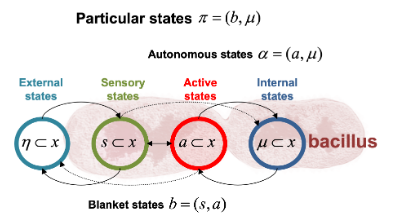
\includegraphics[scale=0.8]{Markov_blankets.png}
   \caption{マルコフブランケット}
   \label{markovblankets}
\end{figure}
{
    \footnotesize
    \noindent
    この影響図は,感覚状態(緑)と能動状態(赤)からなるマルコフブランケットによって区切られた内部状態(青)と外部状態(シアン)への特定の分割を示しています.このグラフのエッジは,条件付き依存関係ではなく,ある状態が別の状態に与える影響を表しています.この図は,単細胞生物に適用されるこの分割を示しています.内部状態は細胞内状態と関連付けられ,感覚状態は表面状態または細胞膜を覆う能動状態(例えば,細胞骨格のアクチンフィラメント)になります.点線は,感覚状態(それぞれ能動状態)から内部状態(それぞれ外部状態)への許容される有向影響を示しています.特定の状態は粒子,すなわち自律状態と感覚状態,あるいはブランケット状態と内部状態を構成します.
}
\subsection{Summary}
要するに,非平衡定常状態の特定の分割は,ある「もの」の内部ダイナミクス(すなわち経路)が,外部経路から条件付き独立であるのは,内部状態の流れが外部状態に依存せず,その逆もまた然りである場合(初期状態が与えられた場合)にのみ起こることを意味します.我々はこれを,何かが存在するための必要十分条件,つまり他のすべてから区別できるという意味で,必要な条件と見なします.初期状態がNESS密度からサンプリングされるとき,特定のソレノイド流の制約の下で,内部状態は外部状態から条件付き独立になります(ブランケット状態が与えられた場合).図\ref{markovblankets}は,結果として生じる特定の分割を示しています.このグラフのエッジが,条件付き依存関係ではなく,ある状態から別の状態への影響を表していることに注意することが重要です.これは,有向影響が条件付き独立性を許容するため重要です.これらの条件付き独立性は,疎で有向なダイナミクスの結合から継承されるヘッセ行列のゼロエントリとして現れます.

\section{From self-organisation to self-evidencing}
特定の分割を装備することで、我々は「もの」について、その内部状態とマルコフ境界、すなわち特定状態—粒子の状態—の観点から語ることができます。次のステップは、自律状態(粒子、植物、または人物)の流れと外部状態との関係を特徴づけることです。言い換えれば、我々は粒子内部と外部の間の結合の性質、つまりそのマルコフブランケットを越えた結合を考慮します。この時点で、我々は特定の分割を持つシステムの特別な領域である(ベイズ)力学へと移行します。

特定の分割の存在は、感覚状態が与えられると—外部状態の条件付き密度を最も可能性の高い内部状態によってパラメーター化されたものとして定義できることを意味します \[7\]。これを、内部モード $\mu(\tau)$ によってパラメーター化された変分密度と呼びます。

$$
q_{\mu}(\eta) \hat{=} p(\eta | s) \\
\mathbf{a}(\tau) = (\mathbf{\alpha}(\tau), \mathbf{\mu}(\tau)) \\
\mathbf{\alpha}[\tau] = \operatorname{arg\,min}_{\alpha} \mathcal{I}(\mathbf{\alpha}[\tau] | s(\tau)) \Rightarrow \\
\mathbf{a}[\tau] = \operatorname{arg\,min}_{\alpha} A(\mathbf{a}[\tau] | \mathbf{s}[\tau]) \Rightarrow \\
\dot{\mathbf{a}}(\tau) = f_a(s, \mathbf{a}) \quad \quad \quad (16)
$$

最小作用の経路と同様に、すべての状態を指定するのに必要な尤度が与えられた場合、モードまたは最も可能性の高い状態を示すために太字を使用します。自律状態の場合、感覚状態のみが必要です。なぜなら、自律状態は外部状態から条件付き独立だからです。

変分密度を誘導することは重要な動きです。これは、すべての感覚状態について、対応する能動モードと内部モード(または能動状態と内部状態の結合空間における自律モード)が存在することを意味します。能動 $a(\tau)$、内部 $\mu(\tau)$、および自律 $a(\tau)$ のモードは、能動、内部、および自律多様体上で進化します。これらの多様体の次元は感覚状態と同じです。我々は後で、これらの多様体が中心多様体としての役割を果たすことを見るでしょう。すなわち、ダイナミクスが指数関数的に発散(または収束)しない多様体です \[13\]。

決定的に、内部多様体も統計的多様体です。なぜなら、その状態が変分密度の十分統計量だからです。これにより、それはメトリックと暗黙的な情報幾何学 \[39, 40, 41\] を備えています。実際、フィッシャー情報計量テンソルは、内部モードの無限小変化から生じるクールバック・ライブラー(KL)ダイバージェンスの変化を測定するものであり、情報距離を導出するリーマン計量です \[42, 付録B\]。これは、内部多様体上のダイナミクスを、外部状態に関するベイズ信念を更新するものと解釈できることを意味します。この解釈は、ベイズ推論の観点から次のように展開できます。

方程式(16)は、すべての感覚状態について、外部状態に関する条件付き密度と、最小の驚きを持つ対応する内部モードが存在することを意味します。このモードは変分密度を指定します。ここで、定義により、変分密度と外部状態に関する条件付き密度の間のKLダイバージェンスはゼロです \[18\]。これは、自律的な流れを変分機能の自由エネルギーに対する勾配の流れとして表現できることを意味します \[19\]。これは(12)から次のようになります。

$$
\begin{bmatrix} f_{\eta}(x) \\ f_{s}(x) \\ f_{a}(\pi) \\ f_{\mu}(\pi) \end{bmatrix} = \Omega \begin{bmatrix} \nabla_{\eta}\mathcal{F}(x) \\ \nabla_{s}\mathcal{F}(x) \\ \nabla_{a}\mathcal{F}(\pi) \\ \nabla_{\mu}\mathcal{F}(\pi) \end{bmatrix} - \Lambda \quad \quad \quad (17)
$$

ここで問題となっている自由エネルギーは、特定の状態の驚きに対する(上限)です。

$$
F(\pi(\tau)) = E_q[\ln q(\eta(\tau)) - \ln p(\eta(\tau)) - \ln p(\pi(\tau) | \eta(\tau))] \\
= E_q[\mathcal{F}(\eta(\tau), \pi(\tau))] - H[q(\eta(\tau))] \\
\text{Expected energy} \quad \quad \quad \text{Entropy} \\
= E_q[\mathcal{I}(\pi(\tau) | \eta(\tau))] + D[q(\eta(\tau)) || p(\eta(\tau))] \\
\text{-ve Accuracy} \quad \quad \quad \text{Complexity} \\
= D[q(\eta(\tau)) || p(\eta(\tau) | \pi(\tau))] + \mathcal{I}(\pi(\tau)) \\
=0 \\
q = q_{\mu}(\eta) = p(\eta | s) = p(\eta | \pi) \\
E[F(\pi)] = E[\mathcal{I}(\pi)] = H[p(\pi)] \quad \quad \quad (18)
$$

この変分自由エネルギーはいくつかの方法で再配置できます。まず、期待エネルギーから変分密度のエントロピーを引いたものとして表現でき、これにより「自由エネルギー」という名前が許容されます \[21\]。この分解では、変分自由エネルギーを最小化することは、期待エネルギーが最小化されるという制約のもとで、最大エントロピー原理に対応します \[46, 47\]。期待エネルギーは、生成モデル、すなわち原因(外部状態)とその結果(特定状態)に関する結合分布としての役割を果たすNESS密度の関数です \[22\]。

第二に、変分自由エネルギーは、特定状態の(負の)対数尤度(つまり、負の正確度)と、事後密度と事前密度の間のKLダイバージェンス(つまり、複雑度)に分解できます。最後に、特定状態に関連する自己情報量(つまり、驚き)と、変分密度と条件付き(つまり、事後)密度の間のKLダイバージェンスの合計として書くことができ、これは構築上ゼロになります。変分ベイズ推論 \[48\] では、負の驚きは、外部状態を周辺化することによって得られる対数周辺尤度またはモデルエビデンス、またはELBO \[49, 44\] と読み替えられます。

では、どのような意味で(17)を推論と解釈できるのでしょうか?自律状態が感覚摂動にどのように応答するか、つまり感覚状態に条件付けられた自律状態の経路を考えてみましょう。感覚状態がゆっくりと変化する場合、自律状態は最も可能性の高い値(つまり、条件付きモード)に向かって流れ、そこに留まります \[23\]。しかし、感覚状態が変化している場合、自律状態は動くターゲットを追跡しようとしているかのように見えます。これは、中心多様体定理 \[13, 50\] に沿って定式化できます。そこでは、中心多様体から離れる(速い)流れと、多様体上の自律モードの(遅い)流れが存在します。

$$
\dot{\varepsilon}(\tau) = \dot{\mathbf{a}}(\tau) - \dot{\alpha}(\tau) = \frac{\partial f_\varepsilon}{\partial \varepsilon} \cdot \varepsilon + \dots = \frac{\partial f_a}{\partial \alpha} \cdot \varepsilon + \dots \\
\Rightarrow \\
\dot{\alpha}(\tau) - \dot{\mathbf{a}}(\tau) = \mathbf{J}_\alpha \cdot (\alpha - \mathbf{a}) + \dots \\
\text{Off manifold flow} \\
= -(\Gamma_{\alpha}\nabla_{\alpha}\mathcal{F}) \cdot (\alpha - \mathbf{a}) + (Q_{\alpha\alpha}\nabla_{\alpha}\mathcal{F}) \cdot (\alpha - \mathbf{a}) + \dots \\
\text{Flow to centre manifold} \quad \quad \quad \text{Flow parallel to the manifold} \quad \quad \quad (21)
$$

これは、展開点での流れがゼロであり、展開の第二項が最初のゼロでない項として残ることを意味します。これは、自律流のヤコビアンが現在の自律状態とそれに対応するモードの間の変位に影響を与えることを示しています。自由エネルギーの二次導関数は、流のヤコビアンから生じます。つまり、(17)を(8)に代入します。したがって、多様体外の流れには、勾配流によって与えられる中心多様体に向かう流れの成分と、ソレノイド流によって与えられる多様体と平行な流れの成分があります。これらを合わせると、図2に示すように、自律状態は中心多様体に向かって常に収束しながら円を描いて流れます。

では、中心多様体上の流れはどうでしょうか?(17)から、自律モードの流れは自由エネルギー勾配の観点から表現できることが分かります。

$$
\dot{\mathbf{a}}(\tau) = (Q_{\alpha\alpha} - \Gamma_{\alpha}) \nabla_a F(s, \mathbf{a}) + \dots \\
= (Q_{\alpha\alpha} - \Gamma_{\alpha}) \nabla_a E_q[\mathcal{I}(s, \mathbf{a} | \eta)] + (Q_{\alpha\alpha} - \Gamma_{\alpha}) \nabla_a D[q_{\mu}(\eta) || p(\eta)] + \dots \\
\text{-ve Accuracy} \quad \quad \quad \text{Complexity} \quad \quad \quad (22)
$$

この表現は、自由エネルギーの精度部分と複雑度部分を分解します。ここで、精度部分は感覚状態に依存し、複雑度部分は自律状態のみに依存します。要するに、中心多様体上の流れは、事前の(ベイズ)信念に従いながら、その予測の精度を最大化しようとしているかのように見えます。ここでいう予測とは、変分密度によって与えられる外部状態に関する事後(ベイズ)信念の下での、期待される感覚状態を指します。

\end{document}